\documentclass[11pt,ignorenonframetext,]{beamer}
\setbeamertemplate{caption}[numbered]
\setbeamertemplate{caption label separator}{: }
\setbeamercolor{caption name}{fg=normal text.fg}
\beamertemplatenavigationsymbolsempty
\usepackage{lmodern}
\usepackage{amssymb,amsmath}
\usepackage{ifxetex,ifluatex}
\usepackage{fixltx2e} % provides \textsubscript
\ifnum 0\ifxetex 1\fi\ifluatex 1\fi=0 % if pdftex
  \usepackage[T1]{fontenc}
  \usepackage[utf8]{inputenc}
\else % if luatex or xelatex
  \ifxetex
    \usepackage{mathspec}
  \else
    \usepackage{fontspec}
  \fi
  \defaultfontfeatures{Ligatures=TeX,Scale=MatchLowercase}
\fi
\usetheme[]{metropolis}
% use upquote if available, for straight quotes in verbatim environments
\IfFileExists{upquote.sty}{\usepackage{upquote}}{}
% use microtype if available
\IfFileExists{microtype.sty}{%
\usepackage{microtype}
\UseMicrotypeSet[protrusion]{basicmath} % disable protrusion for tt fonts
}{}
\newif\ifbibliography
\hypersetup{
            pdftitle={Lecture 19},
            pdfauthor={Colin Rundel},
            pdfborder={0 0 0},
            breaklinks=true}
\urlstyle{same}  % don't use monospace font for urls
\usepackage{color}
\usepackage{fancyvrb}
\newcommand{\VerbBar}{|}
\newcommand{\VERB}{\Verb[commandchars=\\\{\}]}
\DefineVerbatimEnvironment{Highlighting}{Verbatim}{commandchars=\\\{\}}
% Add ',fontsize=\small' for more characters per line
\newenvironment{Shaded}{}{}
\newcommand{\KeywordTok}[1]{\textcolor[rgb]{0.00,0.44,0.13}{\textbf{#1}}}
\newcommand{\DataTypeTok}[1]{\textcolor[rgb]{0.56,0.13,0.00}{#1}}
\newcommand{\DecValTok}[1]{\textcolor[rgb]{0.25,0.63,0.44}{#1}}
\newcommand{\BaseNTok}[1]{\textcolor[rgb]{0.25,0.63,0.44}{#1}}
\newcommand{\FloatTok}[1]{\textcolor[rgb]{0.25,0.63,0.44}{#1}}
\newcommand{\ConstantTok}[1]{\textcolor[rgb]{0.53,0.00,0.00}{#1}}
\newcommand{\CharTok}[1]{\textcolor[rgb]{0.25,0.44,0.63}{#1}}
\newcommand{\SpecialCharTok}[1]{\textcolor[rgb]{0.25,0.44,0.63}{#1}}
\newcommand{\StringTok}[1]{\textcolor[rgb]{0.25,0.44,0.63}{#1}}
\newcommand{\VerbatimStringTok}[1]{\textcolor[rgb]{0.25,0.44,0.63}{#1}}
\newcommand{\SpecialStringTok}[1]{\textcolor[rgb]{0.73,0.40,0.53}{#1}}
\newcommand{\ImportTok}[1]{#1}
\newcommand{\CommentTok}[1]{\textcolor[rgb]{0.38,0.63,0.69}{\textit{#1}}}
\newcommand{\DocumentationTok}[1]{\textcolor[rgb]{0.73,0.13,0.13}{\textit{#1}}}
\newcommand{\AnnotationTok}[1]{\textcolor[rgb]{0.38,0.63,0.69}{\textbf{\textit{#1}}}}
\newcommand{\CommentVarTok}[1]{\textcolor[rgb]{0.38,0.63,0.69}{\textbf{\textit{#1}}}}
\newcommand{\OtherTok}[1]{\textcolor[rgb]{0.00,0.44,0.13}{#1}}
\newcommand{\FunctionTok}[1]{\textcolor[rgb]{0.02,0.16,0.49}{#1}}
\newcommand{\VariableTok}[1]{\textcolor[rgb]{0.10,0.09,0.49}{#1}}
\newcommand{\ControlFlowTok}[1]{\textcolor[rgb]{0.00,0.44,0.13}{\textbf{#1}}}
\newcommand{\OperatorTok}[1]{\textcolor[rgb]{0.40,0.40,0.40}{#1}}
\newcommand{\BuiltInTok}[1]{#1}
\newcommand{\ExtensionTok}[1]{#1}
\newcommand{\PreprocessorTok}[1]{\textcolor[rgb]{0.74,0.48,0.00}{#1}}
\newcommand{\AttributeTok}[1]{\textcolor[rgb]{0.49,0.56,0.16}{#1}}
\newcommand{\RegionMarkerTok}[1]{#1}
\newcommand{\InformationTok}[1]{\textcolor[rgb]{0.38,0.63,0.69}{\textbf{\textit{#1}}}}
\newcommand{\WarningTok}[1]{\textcolor[rgb]{0.38,0.63,0.69}{\textbf{\textit{#1}}}}
\newcommand{\AlertTok}[1]{\textcolor[rgb]{1.00,0.00,0.00}{\textbf{#1}}}
\newcommand{\ErrorTok}[1]{\textcolor[rgb]{1.00,0.00,0.00}{\textbf{#1}}}
\newcommand{\NormalTok}[1]{#1}
\usepackage{graphicx,grffile}
\makeatletter
\def\maxwidth{\ifdim\Gin@nat@width>\linewidth\linewidth\else\Gin@nat@width\fi}
\def\maxheight{\ifdim\Gin@nat@height>\textheight0.8\textheight\else\Gin@nat@height\fi}
\makeatother
% Scale images if necessary, so that they will not overflow the page
% margins by default, and it is still possible to overwrite the defaults
% using explicit options in \includegraphics[width, height, ...]{}
\setkeys{Gin}{width=\maxwidth,height=\maxheight,keepaspectratio}

% Prevent slide breaks in the middle of a paragraph:
\widowpenalties 1 10000
\raggedbottom

\AtBeginPart{
  \let\insertpartnumber\relax
  \let\partname\relax
  \frame{\partpage}
}
\AtBeginSection{
  \ifbibliography
  \else
    \let\insertsectionnumber\relax
    \let\sectionname\relax
    \frame{\sectionpage}
  \fi
}
\AtBeginSubsection{
  \let\insertsubsectionnumber\relax
  \let\subsectionname\relax
  \frame{\subsectionpage}
}

\setlength{\parindent}{0pt}
\setlength{\parskip}{6pt plus 2pt minus 1pt}
\setlength{\emergencystretch}{3em}  % prevent overfull lines
\providecommand{\tightlist}{%
  \setlength{\itemsep}{0pt}\setlength{\parskip}{0pt}}
\setcounter{secnumdepth}{0}

\usepackage{geometry}
\usepackage{graphicx}
\usepackage{amssymb}
\usepackage{color}          	% gives color options
\usepackage{url}		% produces hyperlinks
\usepackage[english]{babel}
\usepackage{colortbl}	% allows for color usage in tables
\usepackage{multirow}	% allows for rows that span multiple rows in tables
\usepackage{xcolor}		% this package has a variety of color options
\usepackage{calc}
\usepackage{multicol}
\usepackage{wrapfig}
\usepackage{textcomp}
\usepackage{bm}
\usepackage{bbm}
\usepackage{setspace}
\usepackage{changepage}
\singlespacing

\usepackage{fontspec}
\newfontfamily\DejaSans{DejaVu Sans}

%%%%%%%%%%%%%%%%
% Small code output
%%%%%%%%%%%%%%%%

%% change fontsize of R code

\makeatletter
\@ifundefined{Shaded}{\newenvironment{Shaded}{}{}}{}
\makeatother


\let\oldShaded\Shaded
\let\endoldShaded\endShaded
\renewenvironment{Shaded}{\footnotesize\begin{spacing}{0.9}\oldShaded}{\endoldShaded\end{spacing}}

%% change fontsize of output
\let\oldverbatim\verbatim
\let\endoldverbatim\endverbatim
\renewenvironment{verbatim}{\footnotesize\begin{spacing}{0.9}\oldverbatim}{\endoldverbatim\end{spacing}}


\newcommand{\tinyoutput}{
  \renewenvironment{Shaded}{\tiny\begin{spacing}{0.9}\oldShaded}{\endoldShaded\end{spacing}}
  \renewenvironment{verbatim}{\tiny\begin{spacing}{0.9}\oldverbatim}{\endoldverbatim\end{spacing}}
}

\newcommand{\scriptoutput}{
  \renewenvironment{Shaded}{\scriptsize\begin{spacing}{0.9}\oldShaded}{\endoldShaded\end{spacing}}
  \renewenvironment{verbatim}{\scriptsize\begin{spacing}{0.9}\oldverbatim}{\endoldverbatim\end{spacing}}
}

\newcommand{\footnoteoutput}{
  \renewenvironment{Shaded}{\footnotesize\begin{spacing}{0.9}\oldShaded}{\endoldShaded\end{spacing}}
  \renewenvironment{verbatim}{\footnotesize\begin{spacing}{0.9}\oldverbatim}{\endoldverbatim\end{spacing}}
}

%\newcommand{\verbatimfont}[1]{\renewcommand{\verbatim@font}{\ttfamily#1}}


%%%%%%%%%%%%%%%%
% Custom Colors
%%%%%%%%%%%%%%%%

\xdefinecolor{oiBlue}{rgb}{0.15, 0.35, 0.55}
\xdefinecolor{gray}{rgb}{0.5, 0.5, 0.5}
\xdefinecolor{darkGray}{rgb}{0.3, 0.3, 0.3}
\xdefinecolor{darkerGray}{rgb}{0.2, 0.2, 0.2}
\xdefinecolor{rubineRed}{rgb}{0.89,0,0.30}
\xdefinecolor{linkCol}{rgb}{0.11,0.49,0.95}	
\xdefinecolor{irishGreen}{rgb}{0,0.60,0}	
\xdefinecolor{darkturquoise}{rgb}{0.44, 0.58, 0.86}
\definecolor{lightGreen}{rgb}{0.533,0.765,0.42}
%\xdefinecolor{hlblue}{rgb}{0.051,0.65,1}
\xdefinecolor{hlblue}{rgb}{ 0.055, 0.639, 0.831}
\definecolor{light}{rgb}{.337,.608,.741}
\definecolor{dark}{rgb}{.337,.608,.741}

\definecolor{cpink}{rgb}{0.93, 0.23, 0.51}

%%%%%%%%%%%%%%%%
% Custom Commands
%%%%%%%%%%%%%%%%

% text colors
\newcommand{\red}[1]{\textit{\textcolor{rubineRed}{#1}}}
\newcommand{\orange}[1]{\textit{\textcolor{orange}{#1}}}
\newcommand{\pink}[1]{\textit{\textcolor{rubineRed!90!white!50}{#1}}}
\newcommand{\green}[1]{\textit{\textcolor{irishGreen}{#1}}}
\newcommand{\blue}[1]{\textit{\textcolor{darkturquoise}{#1}}}
\newcommand{\light}[1]{\textcolor{light}{\textbf{#1}}}
\newcommand{\dark}[1]{\textcolor{dark}{#1}}
\newcommand{\gray}[1]{\textcolor{gray}{#1}}


% links: webURL, webLin, appLink
\newcommand{\webURL}[1]{\urlstyle{same}{\textit{\textcolor{linkCol}{\url{#1}}} }}
\newcommand{\webLink}[2]{\href{#1}{\textcolor{linkCol}{{#2}}}}
\newcommand{\appLink}[2]{\href{#1}{\textcolor{lightGreen!80!black!90}{{#2}}}}

% mail
\newcommand{\mail}[1]{\href{mailto:#1}{\textit{\textcolor{linkCol}{#1}}}}

% highlighting: hl, hlGr, mathhl
\newcommand{\hl}[1]{\textit{\textcolor{hlblue}{#1}}}
\newcommand{\hlGr}[1]{\textit{\textcolor{lightGreen}{#1}}}
\newcommand{\hlRd}[1]{\textit{\textcolor{rubineRed}{#1}}}
\newcommand{\mathhl}[1]{\textcolor{hlblue}{\ensuremath{#1}}}

% example
\newcommand{\ex}[1]{\textcolor{blue}{{{\small (#1)}}}}


\DeclareMathOperator*{\argmin}{arg\,min}
\DeclareMathOperator*{\argmax}{arg\,max}

\title{Lecture 19}
\subtitle{Fitting CAR and SAR Models}
\author{Colin Rundel}
\date{03/29/2017}

\begin{document}
\frame{\titlepage}

\section{Fitting areal models}\label{fitting-areal-models}

\begin{frame}{CAR vs SAR}

\begin{itemize}
\tightlist
\item
  Simultaneous Autogressve (SAR)
\end{itemize}

\[ y(s_i) = \phi \sum_{j=1}^n W_{ij} ~ y(s_j) + \epsilon \]

\[ \bm{y} \sim \mathcal{N}(0,~\sigma^2 \, ((\bm{I}-\phi \bm{W})^{-1}) ((\bm{I}-\phi \bm{W})^{-1})^t )\]

\begin{itemize}
\tightlist
\item
  Conditional Autoregressive (CAR)
\end{itemize}

\[ y(s_i)|\bm{y}_{-s_i} \sim \mathcal{N}\left(\phi\sum_{j=1}^n {W}_{ij} ~ y(s_j),~ \sigma^2 \right) \]

\[ \bm{y} \sim \mathcal{N}(0,~\sigma^2 \, (\bm{I}-\phi \bm{W})^{-1})\]

\end{frame}

\begin{frame}[t]{Some specific generalizations}

Generally speaking we will want to work with a scaled / normalized
version of the weight matrix,
\[ \frac{W_{ij}}{W_{i\boldsymbol{\cdot}}}  \]

\vspace{6mm}

When \(W\) is an adjacency matrix we can express this as
\[ \bm{D}^{-1} \bm{W} \] where \(\bm{D} = \text{diag}(m_i)\) and
\(m_i = |N(s_i)|\).

\vspace{6mm}

We can also allow \(\sigma^2\) to vary between locations, we can define
this as \(\bm{D}_\tau = \text{diag}(1/\sigma^2_i)\) and most often we
use
\[ \bm{D}_\tau = \text{diag}\left(\frac{1}{\sigma^2 / |N(s_i)|}\right) = \bm{D} / \sigma^2  \]
where \(\bm{D}\) is as defined above.

\end{frame}

\begin{frame}[t]{Revised CAR Model}

\begin{itemize}
\tightlist
\item
  Conditional Model
\end{itemize}

\[ y(s_i)|\bm{y}_{-s_i} \sim \mathcal{N}\left(X_{i\cdot}\beta + \phi\sum_{j=1}^n \frac{W_{ij}}{D_{ii}} ~ \big(y(s_j)-X_{j\cdot}\beta\big),~ \sigma^2 D^{-1}_{ii} \right) \]

\vspace{6mm}

\begin{itemize}
\tightlist
\item
  Joint Model
\end{itemize}

\[ \begin{aligned}
\bm{y} &\sim \mathcal{N}(\bm{X}\bm{\beta},~\Sigma_{CAR}) \\
\\
\Sigma_{CAR}
  &= (\bm{D}_{\sigma} \, (\bm{I}-\phi \bm{D}^{-1}\bm{W}))^{-1} \\
  &= (1/\sigma^2 \bm{D} \, (\bm{I}-\phi \bm{D}^{-1}\bm{W}))^{-1} \\
  &= (1/\sigma^2 (\bm{D}-\phi \bm{W}))^{-1} \\
  &= \sigma^2(\bm{D}-\phi \bm{W})^{-1}
\end{aligned}
\]

\end{frame}

\begin{frame}[t]{Revised SAR Model}

\begin{itemize}
\tightlist
\item
  Formula Model
\end{itemize}

\[ y(s_i) = X_{i\cdot}\beta + \phi \sum_{j=1}^n D^{-1}_{jj} \, W_{ij} \, \big(y(s_j) - X_{j\cdot}\beta\big) + \epsilon_i \]

\vspace{6mm}

\begin{itemize}
\tightlist
\item
  Joint Model
\end{itemize}

\[
\begin{aligned}
\bm{y} = \bm{X}\bm{\beta} + \phi \bm{D}^{-1} \bm{W} ~\big(\bm{y}-\bm{X}\bm\beta\big) + \bm{\epsilon} \\
\big(\bm{y}-\bm{X}\bm{\beta}\big) = \phi \bm{D}^{-1} \bm{W} ~\big(\bm{y}-\bm{X}\bm\beta\big) + \bm{\epsilon} \\
\big(\bm{y}-\bm{X}\bm{\beta}\big)(\bm{I}-\phi\bm{D}^{-1}\bm{W})^{-1} = \bm{\epsilon} \\
\bm{y} = \bm{X}\bm{\beta} + (\bm{I} - \phi \bm{D}^{-1} \bm{W})^-1 \bm\epsilon
\end{aligned}
\]

\[
\bm{y} \sim \mathcal{N}\left(\bm{X}\bm{\beta}, (\bm{I} - \phi \bm{D}^{-1} \bm{W})^{-1} \sigma^2 \bm{D}^{-1} \big((\bm{I} - \phi \bm{D}^{-1} \bm{W})^{-1}\big)^t \right)
\]

\end{frame}

\begin{frame}[t]{Toy CAR Example}

\vspace{-3mm}

\begin{center}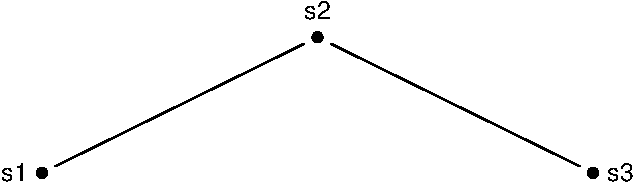
\includegraphics[width=0.6\textwidth]{Lec19_files/figure-beamer/unnamed-chunk-1-1} \end{center}

\pause

\[
\bm{W} = \begin{pmatrix}
0 & 1 & 0 \\
1 & 0 & 1 \\
0 & 1 & 0 
\end{pmatrix}
\qquad\qquad
\bm{D} = \begin{pmatrix}
1 & 0 & 0 \\
0 & 2 & 0 \\
0 & 0 & 1 
\end{pmatrix}
\]

\[
\bm\Sigma = \sigma^2 \, (\bm{D} - \phi \, \bm{W}) = \sigma^2~\begin{pmatrix}
1 & -\phi & 0 \\
-\phi & 2 & -\phi \\
0 & -\phi & 1 
\end{pmatrix}^{-1}
\]

\end{frame}

\begin{frame}[fragile,t]{When does \(\Sigma\) exist?}

\begin{Shaded}
\begin{Highlighting}[]
\NormalTok{check_sigma =}\StringTok{ }\ControlFlowTok{function}\NormalTok{(phi) \{}
\NormalTok{  Sigma_inv =}\StringTok{ }\KeywordTok{matrix}\NormalTok{(}\KeywordTok{c}\NormalTok{(}\DecValTok{1}\NormalTok{,}\OperatorTok{-}\NormalTok{phi,}\DecValTok{0}\NormalTok{,}\OperatorTok{-}\NormalTok{phi,}\DecValTok{2}\NormalTok{,}\OperatorTok{-}\NormalTok{phi,}\DecValTok{0}\NormalTok{,}\OperatorTok{-}\NormalTok{phi,}\DecValTok{1}\NormalTok{), }\DataTypeTok{ncol=}\DecValTok{3}\NormalTok{, }\DataTypeTok{byrow=}\OtherTok{TRUE}\NormalTok{) }
  \KeywordTok{solve}\NormalTok{(Sigma_inv)}
\NormalTok{\}}

\KeywordTok{check_sigma}\NormalTok{(}\DataTypeTok{phi=}\DecValTok{0}\NormalTok{)}
\NormalTok{##      [,1] [,2] [,3]}
\NormalTok{## [1,]    1  0.0    0}
\NormalTok{## [2,]    0  0.5    0}
\NormalTok{## [3,]    0  0.0    1}

\KeywordTok{check_sigma}\NormalTok{(}\DataTypeTok{phi=}\FloatTok{0.5}\NormalTok{)}
\NormalTok{##           [,1]      [,2]      [,3]}
\NormalTok{## [1,] 1.1666667 0.3333333 0.1666667}
\NormalTok{## [2,] 0.3333333 0.6666667 0.3333333}
\NormalTok{## [3,] 0.1666667 0.3333333 1.1666667}

\KeywordTok{check_sigma}\NormalTok{(}\DataTypeTok{phi=}\OperatorTok{-}\FloatTok{0.6}\NormalTok{)}
\NormalTok{##          [,1]     [,2]     [,3]}
\NormalTok{## [1,]  1.28125 -0.46875  0.28125}
\NormalTok{## [2,] -0.46875  0.78125 -0.46875}
\NormalTok{## [3,]  0.28125 -0.46875  1.28125}
\end{Highlighting}
\end{Shaded}

\end{frame}

\begin{frame}[fragile]{}

\begin{Shaded}
\begin{Highlighting}[]
\KeywordTok{check_sigma}\NormalTok{(}\DataTypeTok{phi=}\DecValTok{1}\NormalTok{)}
\NormalTok{## Error in solve.default(Sigma_inv): Lapack routine dgesv: system is exactly singular: U[3,3] = 0}

\KeywordTok{check_sigma}\NormalTok{(}\DataTypeTok{phi=}\OperatorTok{-}\DecValTok{1}\NormalTok{)}
\NormalTok{## Error in solve.default(Sigma_inv): Lapack routine dgesv: system is exactly singular: U[3,3] = 0}

\KeywordTok{check_sigma}\NormalTok{(}\DataTypeTok{phi=}\FloatTok{1.2}\NormalTok{)}
\NormalTok{##            [,1]      [,2]       [,3]}
\NormalTok{## [1,] -0.6363636 -1.363636 -1.6363636}
\NormalTok{## [2,] -1.3636364 -1.136364 -1.3636364}
\NormalTok{## [3,] -1.6363636 -1.363636 -0.6363636}

\KeywordTok{check_sigma}\NormalTok{(}\DataTypeTok{phi=}\OperatorTok{-}\FloatTok{1.2}\NormalTok{)}
\NormalTok{##            [,1]      [,2]       [,3]}
\NormalTok{## [1,] -0.6363636  1.363636 -1.6363636}
\NormalTok{## [2,]  1.3636364 -1.136364  1.3636364}
\NormalTok{## [3,] -1.6363636  1.363636 -0.6363636}
\end{Highlighting}
\end{Shaded}

\end{frame}

\begin{frame}{Conclusions}

Generally speaking just like the AR(1) model for time series we require
that \(|\phi| < 1\) for the CAR model to be proper.

\vspace{4mm}

These results for \(\phi\) also apply in the context where
\(\sigma^2_i\) is constant across locations (i.e.
\(\bm\Sigma = (\sigma^2 \, (\bm{I}-\phi \bm{D}^{-1}\bm{W}))^{-1}\))

\vspace{8mm}

As a side note, the special case where \(\phi=1\) is known as an
intrinsic autoregressive (IAR) model and they are popular as an
\emph{improper} prior for spatial random effects. An additional sum
constraint is necessary for identifiability
(\(\sum{i=1}^n y(s_i) = 0\)).

\end{frame}

\begin{frame}{Example - NC SIDS}

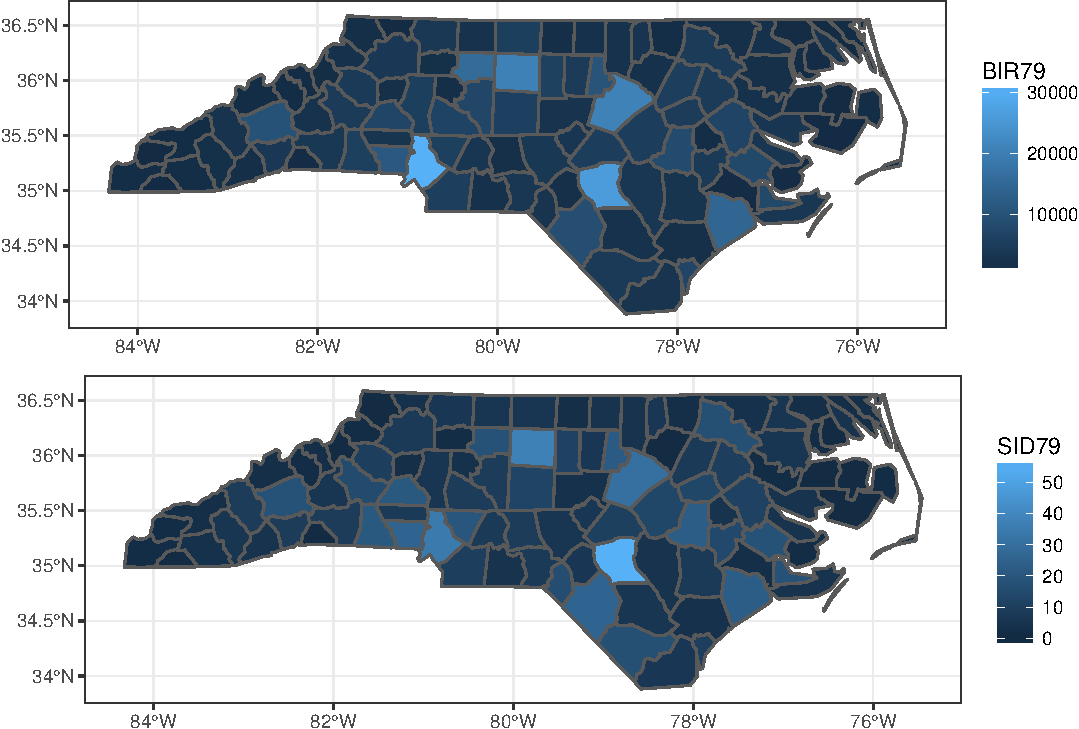
\includegraphics{Lec19_files/figure-beamer/unnamed-chunk-4-1.pdf}

\end{frame}

\begin{frame}[fragile,t]{Using \texttt{spautolm} from \texttt{spdep}}

\begin{Shaded}
\begin{Highlighting}[]
\KeywordTok{library}\NormalTok{(spdep)}

\NormalTok{W =}\StringTok{ }\KeywordTok{st_touches}\NormalTok{(nc, }\DataTypeTok{sparse=}\OtherTok{FALSE}\NormalTok{)}
\NormalTok{listW =}\StringTok{ }\KeywordTok{mat2listw}\NormalTok{(W)}

\NormalTok{listW}
\NormalTok{## Characteristics of weights list object:}
\NormalTok{## Neighbour list object:}
\NormalTok{## Number of regions: 100 }
\NormalTok{## Number of nonzero links: 490 }
\NormalTok{## Percentage nonzero weights: 4.9 }
\NormalTok{## Average number of links: 4.9 }
\NormalTok{## }
\NormalTok{## Weights style: M }
\NormalTok{## Weights constants summary:}
\NormalTok{##     n    nn  S0  S1    S2}
\NormalTok{## M 100 10000 490 980 10696}
\end{Highlighting}
\end{Shaded}

\end{frame}

\begin{frame}[fragile,t]{}

\begin{Shaded}
\begin{Highlighting}[]
\NormalTok{nc_coords =}\StringTok{ }\NormalTok{nc }\OperatorTok\StringTok{ }\KeywordTok{st_centroid}\NormalTok{() }\OperatorTok\StringTok{ }\KeywordTok{st_coordinates}\NormalTok{()}

\KeywordTok{plot}\NormalTok{(}\KeywordTok{st_geometry}\NormalTok{(nc))}
\KeywordTok{plot}\NormalTok{(listW, nc_coords, }\DataTypeTok{add=}\OtherTok{TRUE}\NormalTok{, }\DataTypeTok{col=}\StringTok{"blue"}\NormalTok{, }\DataTypeTok{pch=}\DecValTok{16}\NormalTok{)}
\end{Highlighting}
\end{Shaded}

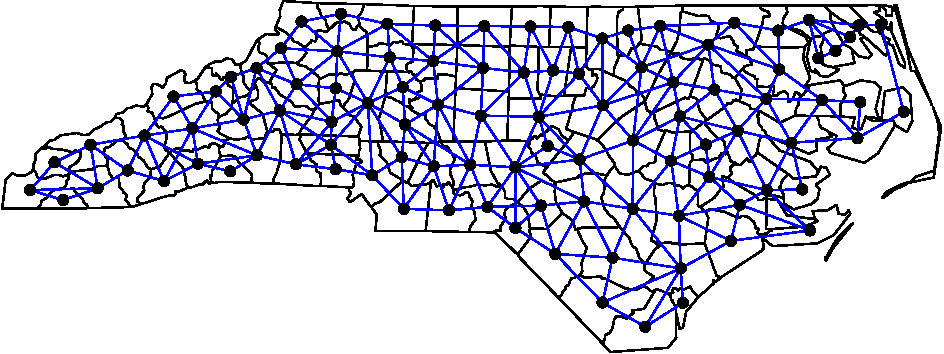
\includegraphics{Lec19_files/figure-beamer/unnamed-chunk-6-1.pdf}

\end{frame}

\begin{frame}[fragile,t]{CAR Model}

\scriptoutput

\begin{Shaded}
\begin{Highlighting}[]
\NormalTok{nc_car =}\StringTok{ }\KeywordTok{spautolm}\NormalTok{(}\DataTypeTok{formula =}\NormalTok{ SID74 }\OperatorTok{~}\StringTok{ }\NormalTok{BIR74, }\DataTypeTok{data =}\NormalTok{ nc, }
                  \DataTypeTok{listw =}\NormalTok{ listW, }\DataTypeTok{family =} \StringTok{"CAR"}\NormalTok{) }

\KeywordTok{summary}\NormalTok{(nc_car)}
\NormalTok{## }
\NormalTok{## Call: }
\NormalTok{## spautolm(formula = SID74 ~ BIR74, data = nc, listw = listW, family = "CAR")}
\NormalTok{## }
\NormalTok{## Residuals:}
\NormalTok{##       Min        1Q    Median        3Q       Max }
\NormalTok{## -10.38934  -1.58600  -0.52154   1.14729  13.54059 }
\NormalTok{## }
\NormalTok{## Coefficients: }
\NormalTok{##               Estimate Std. Error z value Pr(>|z|)}
\NormalTok{## (Intercept) 1.06911902 0.67501301  1.5838   0.1132}
\NormalTok{## BIR74       0.00175249 0.00010107 17.3401   <2e-16}
\NormalTok{## }
\NormalTok{## Lambda: 0.13222 LR test value: 8.8654 p-value: 0.0029062 }
\NormalTok{## Numerical Hessian standard error of lambda: 0.030094 }
\NormalTok{## }
\NormalTok{## Log likelihood: -275.7655 }
\NormalTok{## ML residual variance (sigma squared): 13.695, (sigma: 3.7007)}
\NormalTok{## Number of observations: 100 }
\NormalTok{## Number of parameters estimated: 4 }
\NormalTok{## AIC: 559.53}
\end{Highlighting}
\end{Shaded}

\end{frame}

\begin{frame}[fragile,t]{SAR Model}

\scriptoutput

\begin{Shaded}
\begin{Highlighting}[]
\NormalTok{nc_sar =}\StringTok{ }\KeywordTok{spautolm}\NormalTok{(}\DataTypeTok{formula =}\NormalTok{ SID74 }\OperatorTok{~}\StringTok{ }\NormalTok{BIR74, }\DataTypeTok{data =}\NormalTok{ nc, }
                  \DataTypeTok{listw =}\NormalTok{ listW, }\DataTypeTok{family =} \StringTok{"SAR"}\NormalTok{)}

\KeywordTok{summary}\NormalTok{(nc_sar)}
\NormalTok{## }
\NormalTok{## Call: }
\NormalTok{## spautolm(formula = SID74 ~ BIR74, data = nc, listw = listW, family = "SAR")}
\NormalTok{## }
\NormalTok{## Residuals:}
\NormalTok{##       Min        1Q    Median        3Q       Max }
\NormalTok{## -10.94771  -1.72354  -0.56866   1.23273  14.70511 }
\NormalTok{## }
\NormalTok{## Coefficients: }
\NormalTok{##               Estimate Std. Error z value Pr(>|z|)}
\NormalTok{## (Intercept) 1.01971585 0.64910408   1.571   0.1162}
\NormalTok{## BIR74       0.00174741 0.00010105  17.292   <2e-16}
\NormalTok{## }
\NormalTok{## Lambda: 0.075265 LR test value: 8.4013 p-value: 0.0037495 }
\NormalTok{## Numerical Hessian standard error of lambda: 0.024085 }
\NormalTok{## }
\NormalTok{## Log likelihood: -275.9975 }
\NormalTok{## ML residual variance (sigma squared): 14.158, (sigma: 3.7627)}
\NormalTok{## Number of observations: 100 }
\NormalTok{## Number of parameters estimated: 4 }
\NormalTok{## AIC: 560}
\end{Highlighting}
\end{Shaded}

\end{frame}

\begin{frame}{Residuals}

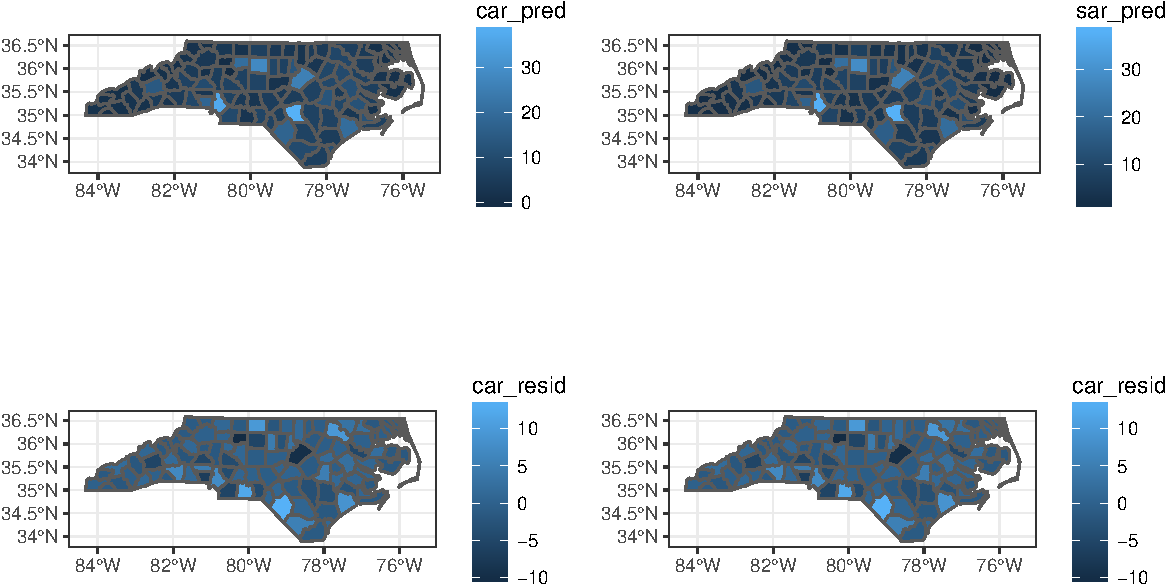
\includegraphics{Lec19_files/figure-beamer/unnamed-chunk-9-1.pdf}

\end{frame}

\begin{frame}{I agree \ldots{}}

\begin{center}

\includegraphics[width=0.8\textwidth]{figs/your-model.jpg}
\end{center}

\end{frame}

\begin{frame}{Why?}

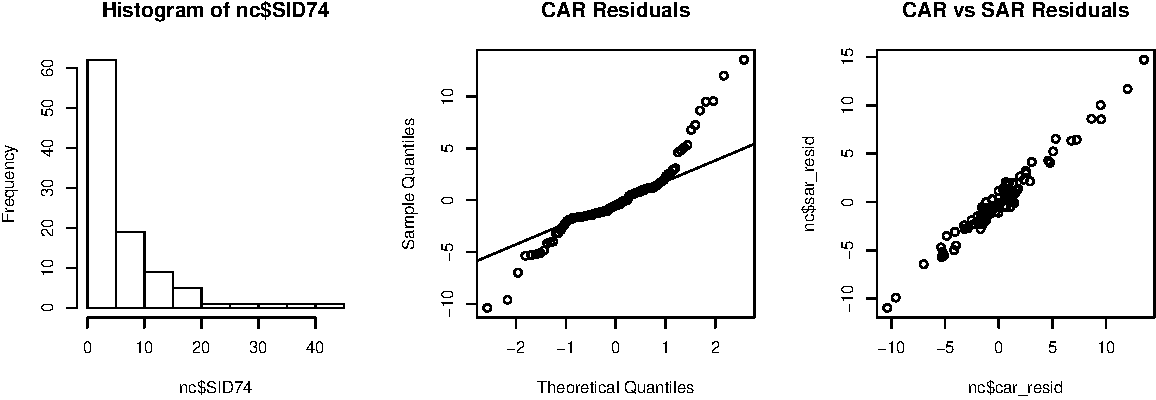
\includegraphics{Lec19_files/figure-beamer/unnamed-chunk-10-1.pdf}

\end{frame}

\begin{frame}[fragile,t]{Jags CAR Model}

\scriptoutput

\begin{verbatim}
## model{
##   y ~ dmnorm(beta0 + beta1*x, tau * (D - phi*W))
##   y_pred ~ dmnorm(beta0 + beta1*x, tau * (D - phi*W))
##   
##   beta0 ~ dnorm(0, 1/100)
##   beta1 ~ dnorm(0, 1/100)
## 
##   tau <- 1 / sigma2
##   sigma2 ~ dnorm(0, 1/100) T(0,)
##   phi ~ dunif(-0.99, 0.99)
## }
\end{verbatim}

\begin{Shaded}
\begin{Highlighting}[]
\NormalTok{y =}\StringTok{ }\NormalTok{nc}\OperatorTok{$}\NormalTok{SID74}
\NormalTok{x =}\StringTok{ }\NormalTok{nc}\OperatorTok{$}\NormalTok{BIR74}

\NormalTok{W =}\StringTok{ }\NormalTok{W }\OperatorTok{*}\StringTok{ }\NormalTok{1L}
\NormalTok{D =}\StringTok{ }\KeywordTok{diag}\NormalTok{(}\KeywordTok{rowSums}\NormalTok{(W))}
\end{Highlighting}
\end{Shaded}

\pause

Why don't we use the conditional definition for the \(y\)'s?

\end{frame}

\begin{frame}{Model Results}

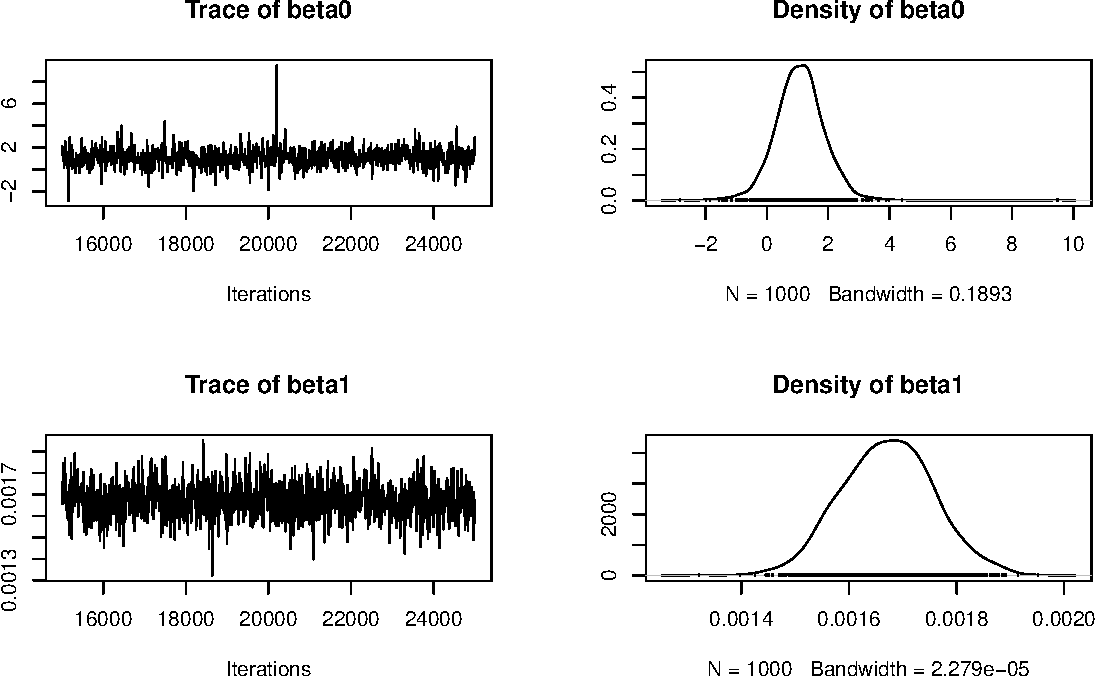
\includegraphics{Lec19_files/figure-beamer/unnamed-chunk-14-1.pdf}

\end{frame}

\begin{frame}{}

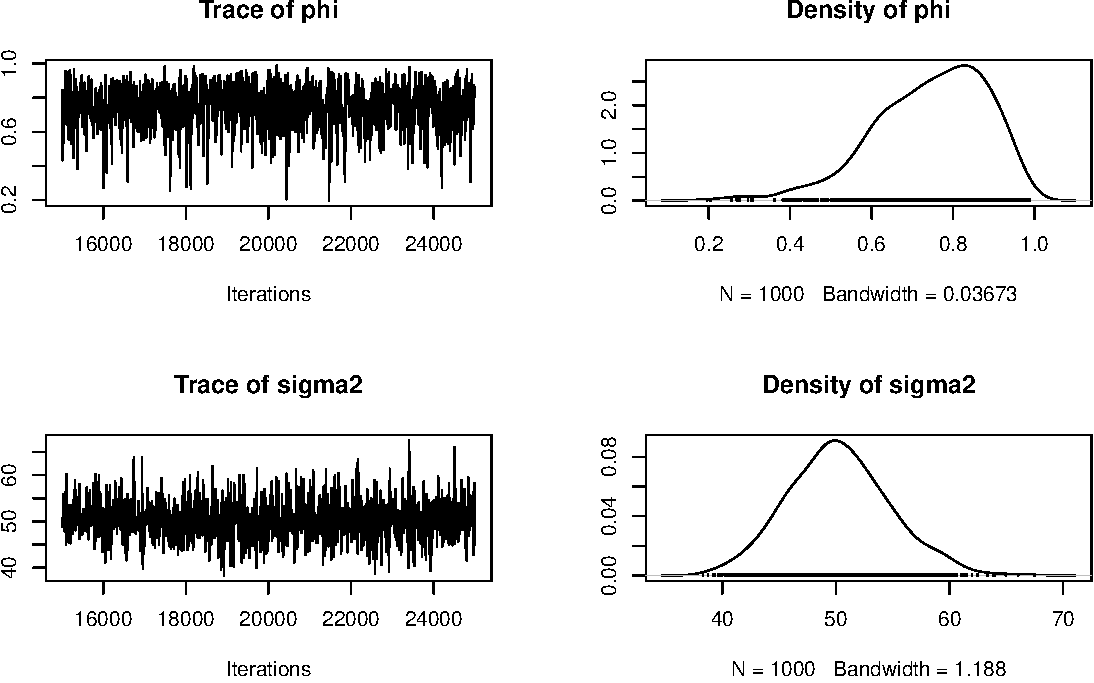
\includegraphics{Lec19_files/figure-beamer/unnamed-chunk-15-1.pdf}

\end{frame}

\begin{frame}[fragile]{Predictions}

\scriptoutput

\begin{Shaded}
\begin{Highlighting}[]
\NormalTok{nc}\OperatorTok{$}\NormalTok{jags_pred =}\StringTok{ }\NormalTok{y_pred}\OperatorTok{$}\NormalTok{post_mean}
\NormalTok{nc}\OperatorTok{$}\NormalTok{jags_resid =}\StringTok{ }\NormalTok{nc}\OperatorTok{$}\NormalTok{SID74 }\OperatorTok{-}\StringTok{ }\NormalTok{y_pred}\OperatorTok{$}\NormalTok{post_mean}

\KeywordTok{sqrt}\NormalTok{(}\KeywordTok{mean}\NormalTok{(nc}\OperatorTok{$}\NormalTok{jags_resid}\OperatorTok{^}\DecValTok{2}\NormalTok{))}
\NormalTok{## [1] 3.987985}
\KeywordTok{sqrt}\NormalTok{(}\KeywordTok{mean}\NormalTok{(nc}\OperatorTok{$}\NormalTok{car_resid}\OperatorTok{^}\DecValTok{2}\NormalTok{))}
\NormalTok{## [1] 3.72107}
\KeywordTok{sqrt}\NormalTok{(}\KeywordTok{mean}\NormalTok{(nc}\OperatorTok{$}\NormalTok{sar_resid}\OperatorTok{^}\DecValTok{2}\NormalTok{))}
\NormalTok{## [1] 3.762664}
\end{Highlighting}
\end{Shaded}

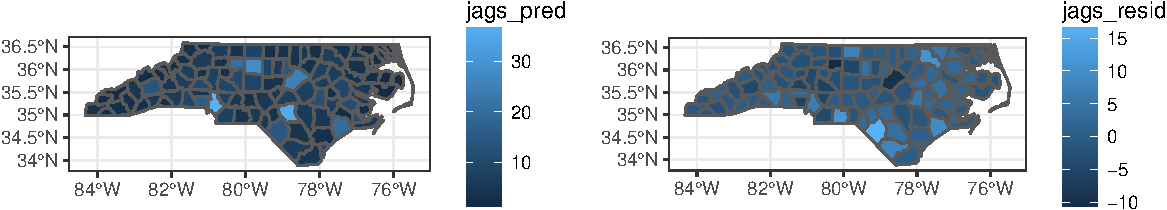
\includegraphics{Lec19_files/figure-beamer/unnamed-chunk-17-1.pdf}

\end{frame}

\begin{frame}{}

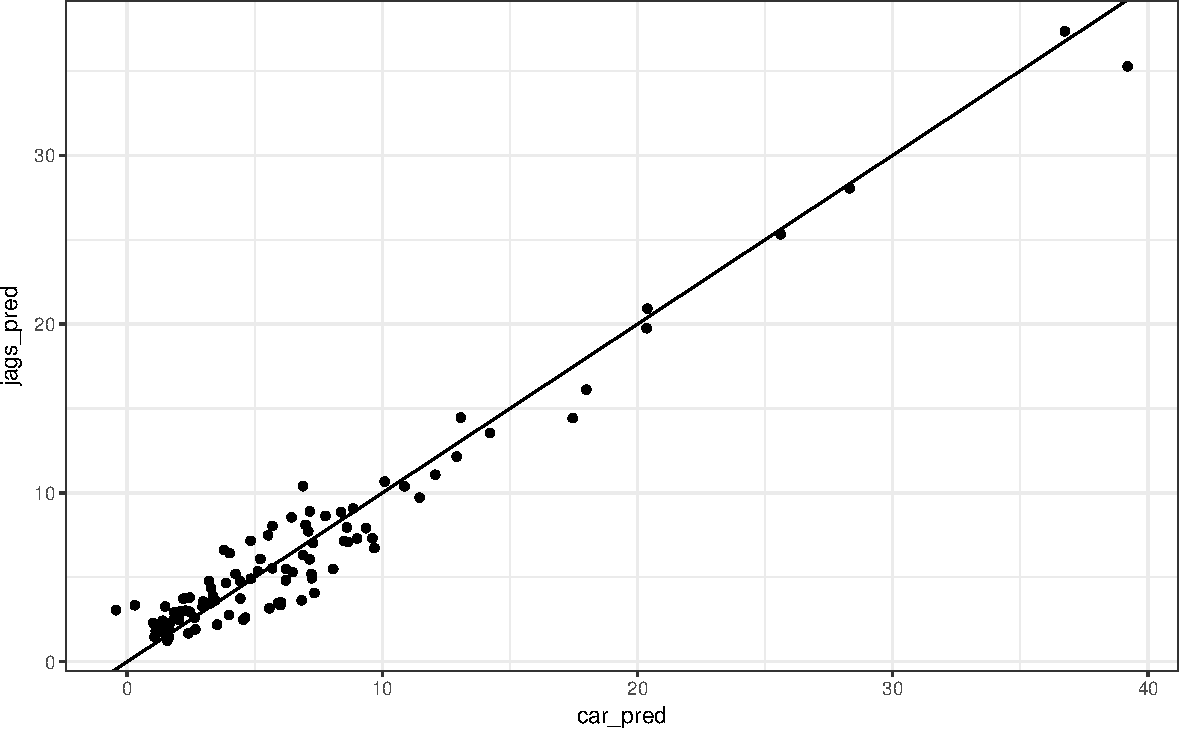
\includegraphics{Lec19_files/figure-beamer/unnamed-chunk-18-1.pdf}

\end{frame}

\begin{frame}{Brief Aside - SAR Precision Matrix}

\[ 
\Sigma_{SAR} = (\bm{I}-\phi \bm{D}^{-1} \, \bm{W})^{-1} \sigma^2 \, \bm{D}^{-1} \left((\bm{I}-\phi \bm{D}^{-1} \, \bm{W})^{-1}\right)^t
\]

\vspace{6mm}

\[ \begin{aligned}
\Sigma^{-1}_{SAR} 
  &= \left( (\bm{I}-\phi \bm{D}^{-1} \, \bm{W})^{-1} \sigma^2 \, \bm{D}^{-1} \left((\bm{I}-\phi \bm{D}^{-1} \, \bm{W})^{-1}\right)^t \right)^{-1} \\
  &= \left( \left( (\bm{I}-\phi \bm{D}^{-1} \, \bm{W})^{-1}\right)^t\right)^{-1} \frac{1}{\sigma^2} \, \bm{D} ~ (\bm{I}-\phi \bm{D}^{-1} \, \bm{W}) \\
  &= \frac{1}{\sigma^2} \, (\bm{I}-\phi \bm{D}^{-1} \, \bm{W})^t ~ \bm{D} ~ (\bm{I}-\phi \bm{D}^{-1} \, \bm{W}) \\
\end{aligned}\]

\end{frame}

\begin{frame}[fragile,t]{Jags SAR Model}

\scriptoutput

\begin{verbatim}
## model{
##   y ~ dmnorm(beta0 + beta1*x, tau * (D - phi*W))
##   y_pred ~ dmnorm(beta0 + beta1*x, tau * (D - phi*W))
##   
##   beta0 ~ dnorm(0, 1/100)
##   beta1 ~ dnorm(0, 1/100)
## 
##   tau <- 1 / sigma2
##   sigma2 ~ dnorm(0, 1/100) T(0,)
##   phi ~ dunif(-0.99, 0.99)
## }
\end{verbatim}

\begin{Shaded}
\begin{Highlighting}[]
\NormalTok{D_inv =}\StringTok{ }\KeywordTok{diag}\NormalTok{(}\DecValTok{1}\OperatorTok{/}\KeywordTok{diag}\NormalTok{(D))}
\NormalTok{W_tilde =}\StringTok{ }\NormalTok{D_inv }\OperatorTok\StringTok{ }\NormalTok{W}
\NormalTok{I =}\StringTok{ }\KeywordTok{diag}\NormalTok{(}\DecValTok{1}\NormalTok{, }\DataTypeTok{ncol=}\KeywordTok{length}\NormalTok{(y), }\DataTypeTok{nrow=}\KeywordTok{length}\NormalTok{(y))}
\end{Highlighting}
\end{Shaded}

\end{frame}

\begin{frame}{Model Results}

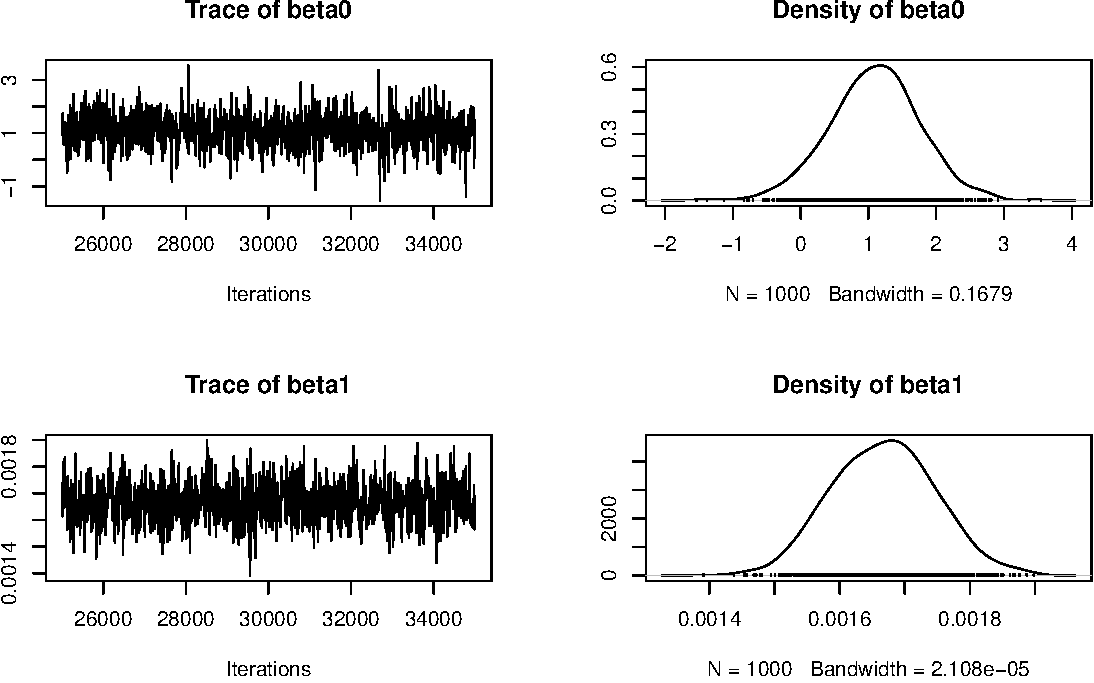
\includegraphics{Lec19_files/figure-beamer/unnamed-chunk-22-1.pdf}

\end{frame}

\begin{frame}{}

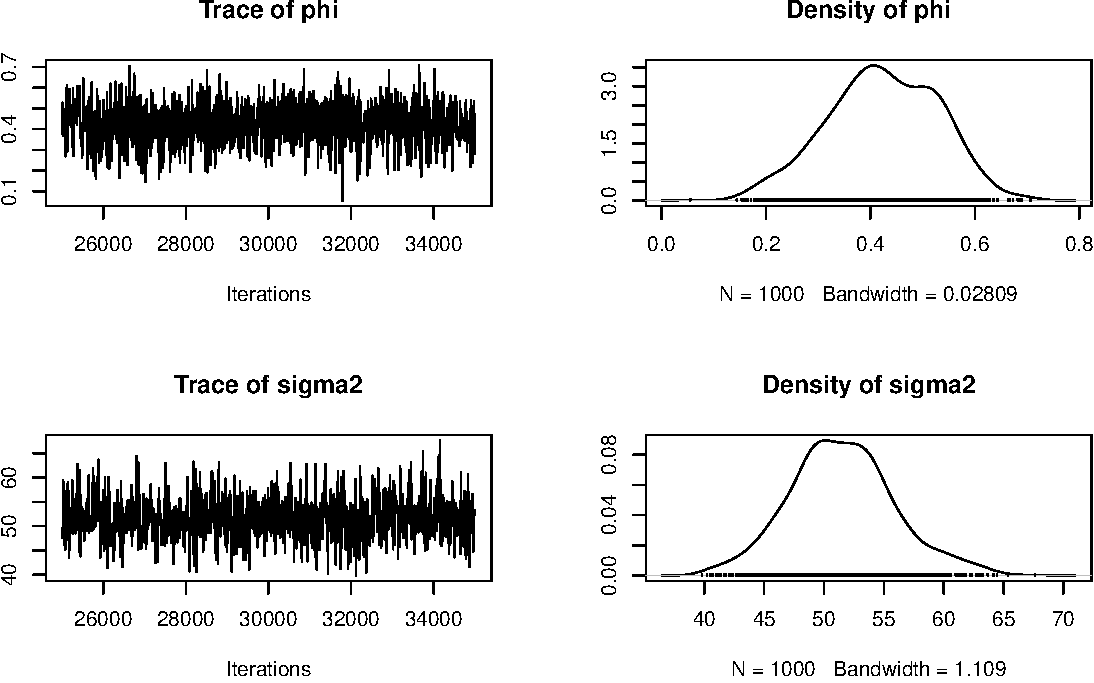
\includegraphics{Lec19_files/figure-beamer/unnamed-chunk-23-1.pdf}

\end{frame}

\begin{frame}{Comparing Model Results}

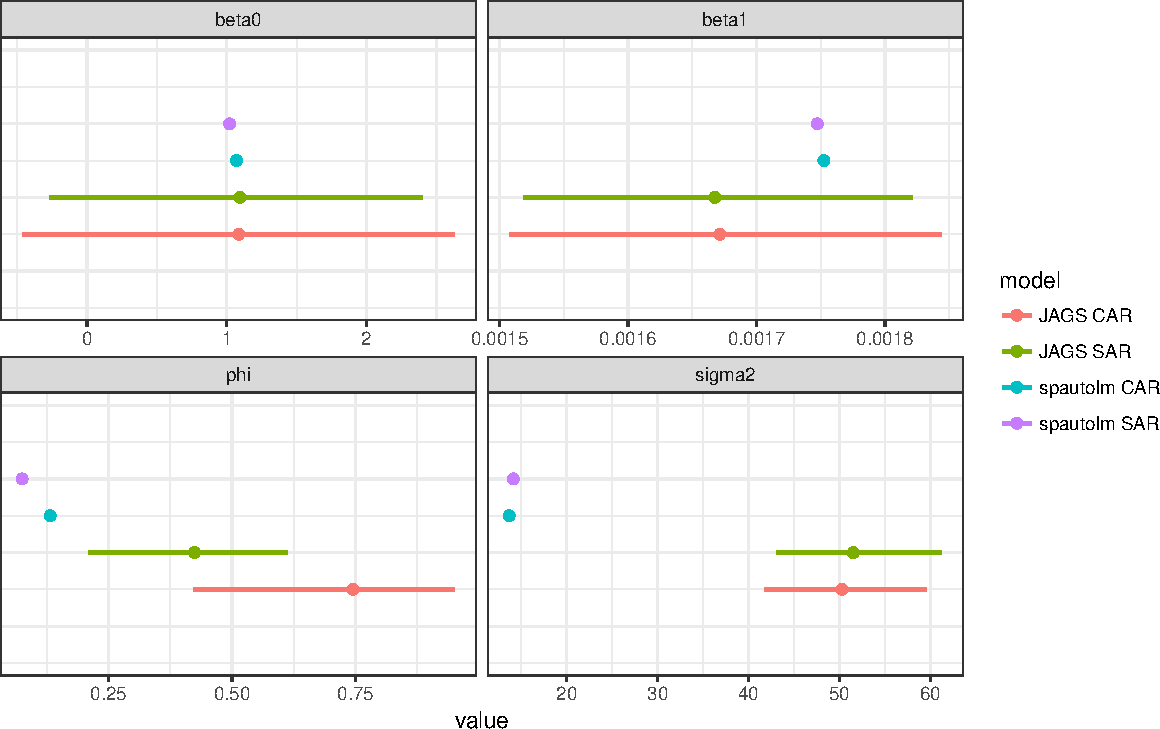
\includegraphics{Lec19_files/figure-beamer/unnamed-chunk-24-1.pdf}

\end{frame}

\end{document}
